\chapter{Introduction and Background} \label{Chap2}
\pagenumbering{arabic}

Quantum computers are expected to surpass classical computers in processing complex data, potentially revolutionizing various fields such as quantum chemistry \cite{Cao2019}, machine learning \cite{paler_machine_2023}, and quantum simulation \cite{peruzzo_variational_2014}. Currently, quantum computing is in the Noisy Intermediate-Scale Quantum (NISQ) era, characterized by quantum processors with tens to hundreds of qubits \cite{preskill_quantum_2018}. To expand the number of qubits, both academic and industrial efforts are shifting towards utilizing quantum networks to link multiple smaller quantum chips. However, significant challenges exist in connecting multiple quantum computers and executing circuits across them simultaneously, along with algorithmic difficulties due to device limitations. This project will focus on simulating qubit placement on physical devices and incorporating swap gates to address networked quantum computers connectivity constraints.

\section{Distributed Quantum Computing} % done chat, turnitin
\acrfull{dqc} involves breaking down a large quantum computation into smaller parts that are executed on multiple interconnected processors, rather than relying on a single large quantum computer with many qubits \cite{cuomo_towards_2020}. As shown in Figure \ref{fig:mono-vs-distributed}, this approach uses smaller quantum devices, each with a limited number of qubits, working together to perform complex computations. In this system, qubits can be shared and entangled between different quantum processors across a network, allowing the execution of quantum algorithms that require more resources than any single quantum processor could handle on its own. A primary goal in \acrshort{dqc} architecture is to minimize the number of operations, including connecting gates and interactions between different \acrfull{qpu} \cite{caleffi_distributed_2024}.
\begin{figure}[htb]
    \centering
    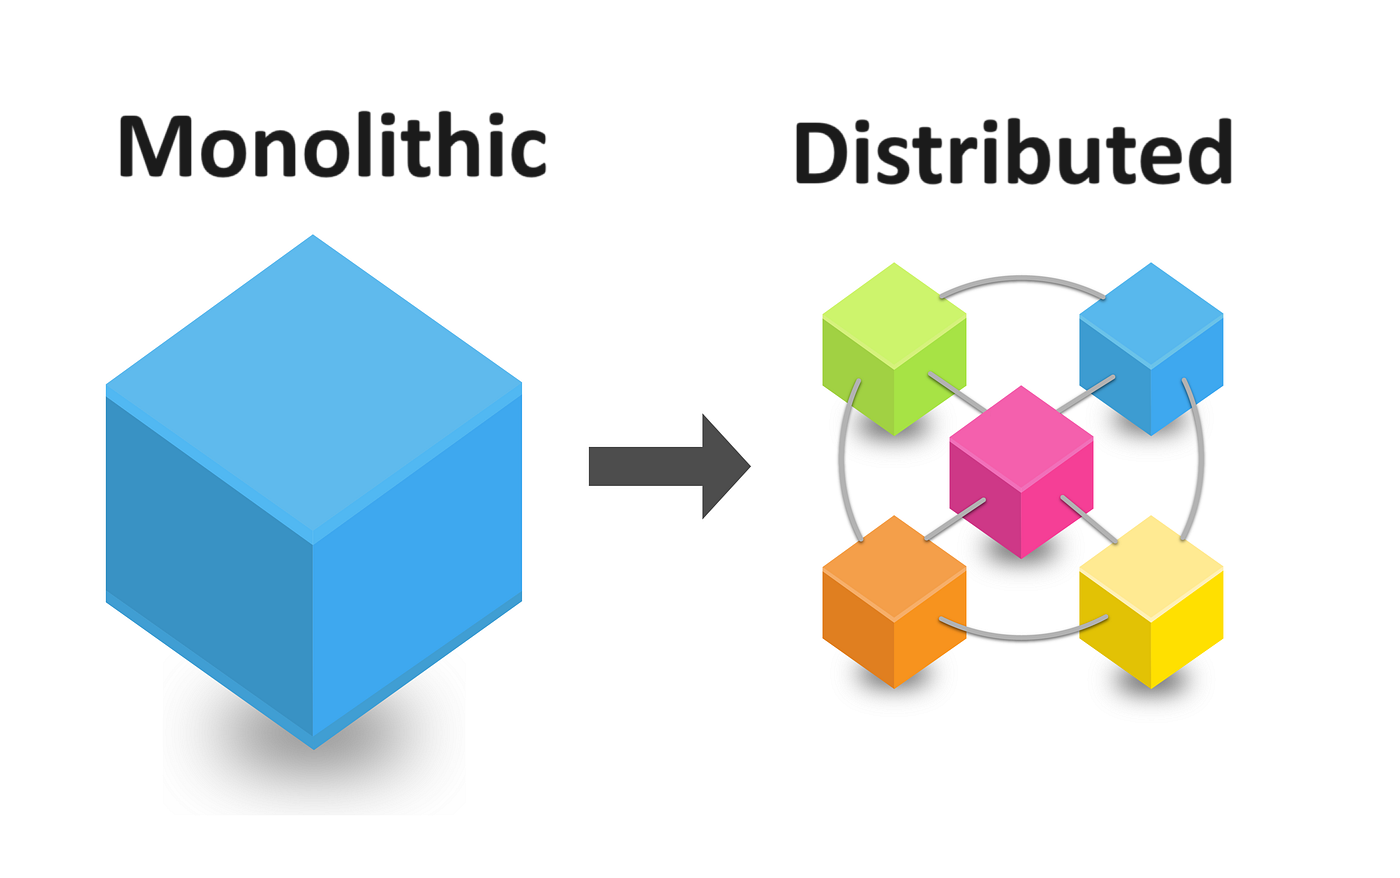
\includegraphics[width=0.4\linewidth]{image/mono vs distributed.png}
    \caption{Monolithic versus distributed illustration. Adapted from \cite{boroglu_microservices_2024}}
    \label{fig:mono-vs-distributed}
\end{figure}

\newpage
\section{Quantum Computing Architecture} % done chat, edited from turnitin, not yet checked for copy again
Gate-based quantum computing is the foundation of most quantum computing architectures today. These systems rely on a limited set of native quantum gates, including single-qubit gates (such as Pauli-X, Y, Z, Hadamard, and phase gates) and two-qubit gates like the Controlled-NOT (CNOT) gate. While single-qubit gates can be applied directly to qubits, a CNOT gate requires the qubits to be adjacent on the coupling map. Despite the limited number of these gates, any quantum circuit can be constructed by carefully combining these operations \cite{barenco_elementary_1995}. This universality is a key aspect of quantum computing, enabling the design and execution of complex quantum algorithms within the constraints of available gate sets. \\
However, implementing these gates physically presents challenges, especially regarding qubit connectivity. In some quantum platforms, such as those using superconducting qubits \cite{krantz_quantum_2019}, the connectivity between qubits is constrained by the architecture's coupling graph. This graph defines the possible interactions between qubits, meaning not all qubits can directly interact with each other through two-qubit gates. As a result, additional operations, such as swap gates, may be needed to bring qubits into positions where the desired two-qubit gate can be applied. This added complexity can affect the efficiency and fidelity of quantum circuits, especially as the scale of the computation grows \cite{khandavilli_towards_2023}. \\
In this context, it is important to distinguish between logical qubits and physical qubits. According to \citeauthor{itoko_optimization_2020}, logical qubits refer to the abstract entities on which quantum algorithms and operations are defined (different from the concept of logical qubits in quantum error correction). These qubits exist independently of the physical hardware, representing the idealized qubits that are free from noise and hardware constraints \cite{itoko_optimization_2020}. On the other hand, physical qubits are the actual qubits within a quantum processor where quantum operations are executed. The performance of physical qubits is influenced by hardware limitations such as decoherence, gate fidelity, and connectivity constraints \cite{bandic_interaction_2023}. Understanding the relationship between logical and physical qubits is crucial for effectively mapping quantum algorithms onto real quantum hardware, ensuring that the physical resources are used optimally while minimizing the effect of hardware imperfections. \\
In the 127-qubit IBM quantum system, \textit{ibm\_kyoto} supports four single-qubit gates (ID, RZ, SX, X) and \acrshort{ecr} gates for two-qubit operations. From Figure \ref{fig:ibm-kyoto}, a CNOT operation between $q_1$ and $q_2$ can be executed directly, but between $q_0$ and $q_2$, additional steps are needed. This highlights the requirement of a preliminary circuit preprocessing step, known as \textit{quantum transpiling} \cite{ferrari_compiler_2021}, before running a quantum circuit.
\begin{figure}
    \centering
    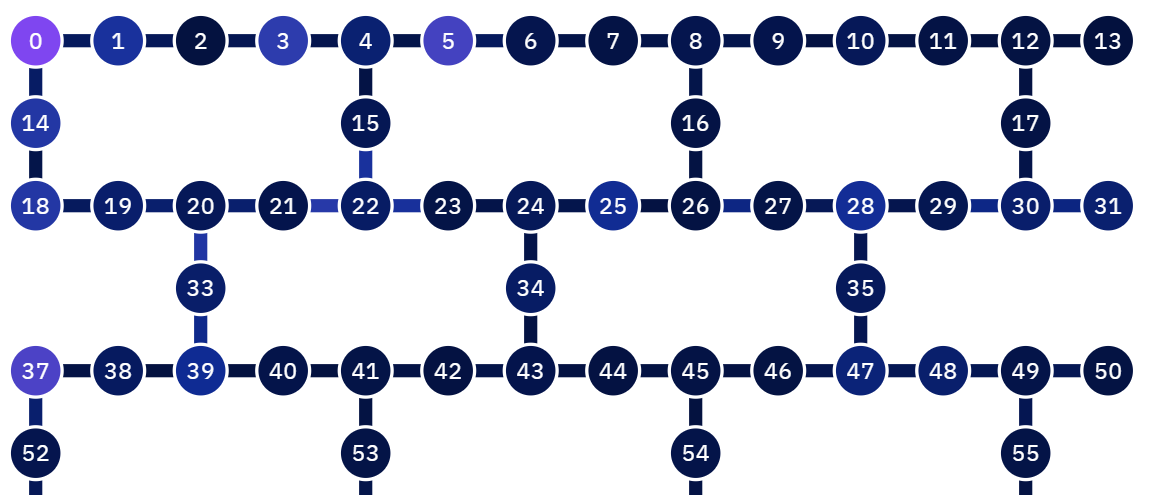
\includegraphics[width=0.6\linewidth]{image/ibm_kyoto.png}
    \caption{Partial coupling map of 127-qubit \textit{ibm\_kyoto}. Adapted from \citeauthor{ibmquantum_computeresources} \protect\cite{ibmquantum_computeresources}. The nodes represent physical qubits, and the edges between nodes represent possible two-qubit gate operations.}
    \label{fig:ibm-kyoto}
\end{figure}

\section{Quantum Circuit Mapping} % done chat, edited from turnitin not yet checked again
A quantum circuit compiler translates a logical quantum circuit into instructions that can be directly executed on a real \acrshort{qpu}. The compiler converts high-level programming languages, like Qiskit in Python \cite{aleksandrowicz_qiskit_2019}, into low-level instructions, such as OpenQASM \cite{cross_open_2017}. Quantum algorithms, as defined in quantum circuits, are generally hardware-agnostic and may not account for specific hardware limitations \cite{ash-saki_qure_2019}. To run these algorithms on a quantum processor, they must be adapted through a process called "quantum circuit mapping" (also known as quantum transpiling), which can increase gate count $(g)$ or circuit depth $(d)$, depending on the circuit and hardware constraints. \\
Figure \ref{fig:tackling-depth-gate-first} presents a 9-qubit device with two CNOT gates: $(q_1, q_2)$ (blue) and $(q_3, q_4)$ (green). The left side shows the original mapping and two different optimization approaches are explained:
\begin{enumerate}[nolistsep]
    \item \textbf{Depth First}: SWAP $(q_2, q_9)$, $(q_1, q_5)$ can be directly performed to connect CNOT $(q_1, q_2)$, and also SWAP $(q_4, q_8)$, $(q_3, q_7)$ to connect CNOT $(q_3, q_4)$. This method adds 4 SWAPs but only increases circuit depth by 1.
    \item \textbf{Gates First}: SWAP $(q_2, q_9)$ is done first, followed by swaps on $(q_2, q_3)$ and $(q_4, q_8)$. This method only adds 3 SWAPs but increases circuit depth by 2.
\end{enumerate} 
\begin{figure}[htb]
    \centering
    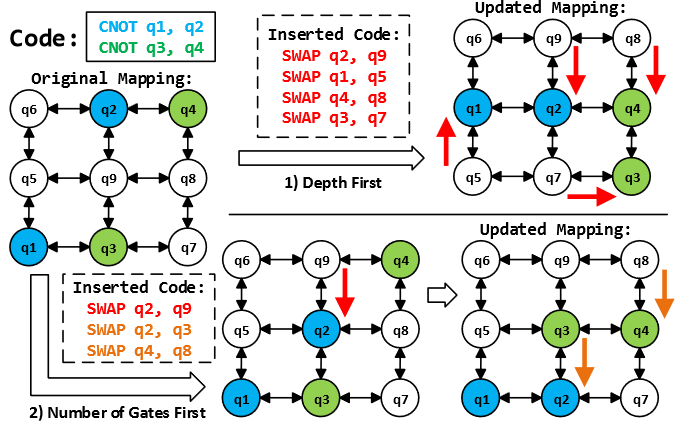
\includegraphics[width=0.6\linewidth]{image/tackling_depth_gate_first.png}
    \caption{Example of a trade-off between depth-first and gate-first. Adapted from \cite{li_tackling_2019}}
    \label{fig:tackling-depth-gate-first}
\end{figure}

\section{Qiskit Framework}
Qiskit is a quantum software program that converts quantum circuits into a format that can be executed on the IBM Quantum Platform \cite{ibmquantum_computeresources}. It utilizes a ``transpilation'' process to transform a given logical circuit to be compatible with a specific target device while also optimizing the circuit to enhance performance and achieve better results.

\subsection{Pass Manager}
The compilation process consists of six stages known as Pass Managers \cite{ibmquantum_transpiler} (Figure \ref{fig:transpiler}), which include:
\begin{enumerate}[nolistsep]
    \item \lstinline{init}: Runs initial passes to prepare the circuit for the backend, including unrolling custom instructions and converting multi-qubit gates into 1- and 2-qubit gates.
    \item \lstinline{layout}: Maps the logical qubits in the circuit to the physical qubits on the target quantum device.
    \item \lstinline{routing}: Inserts SWAP gates into the circuit to align with the physical connectivity of the backend, ensuring qubits that need to interact are adjacent.
    \item \lstinline{translation}: Converts the circuit's gates into the basis gates supported by the target backend, making the circuit executable on the specific hardware.
    \item \lstinline{optimization}: Performs multiple iterations of optimization to reduce circuit depth and gate count until a specified condition, such as a fixed depth, is met.
    \item \lstinline{scheduling}: Manages the timing and order of gate executions on the hardware to ensure optimal performance during execution.
    \begin{figure}[h]
        \centering
        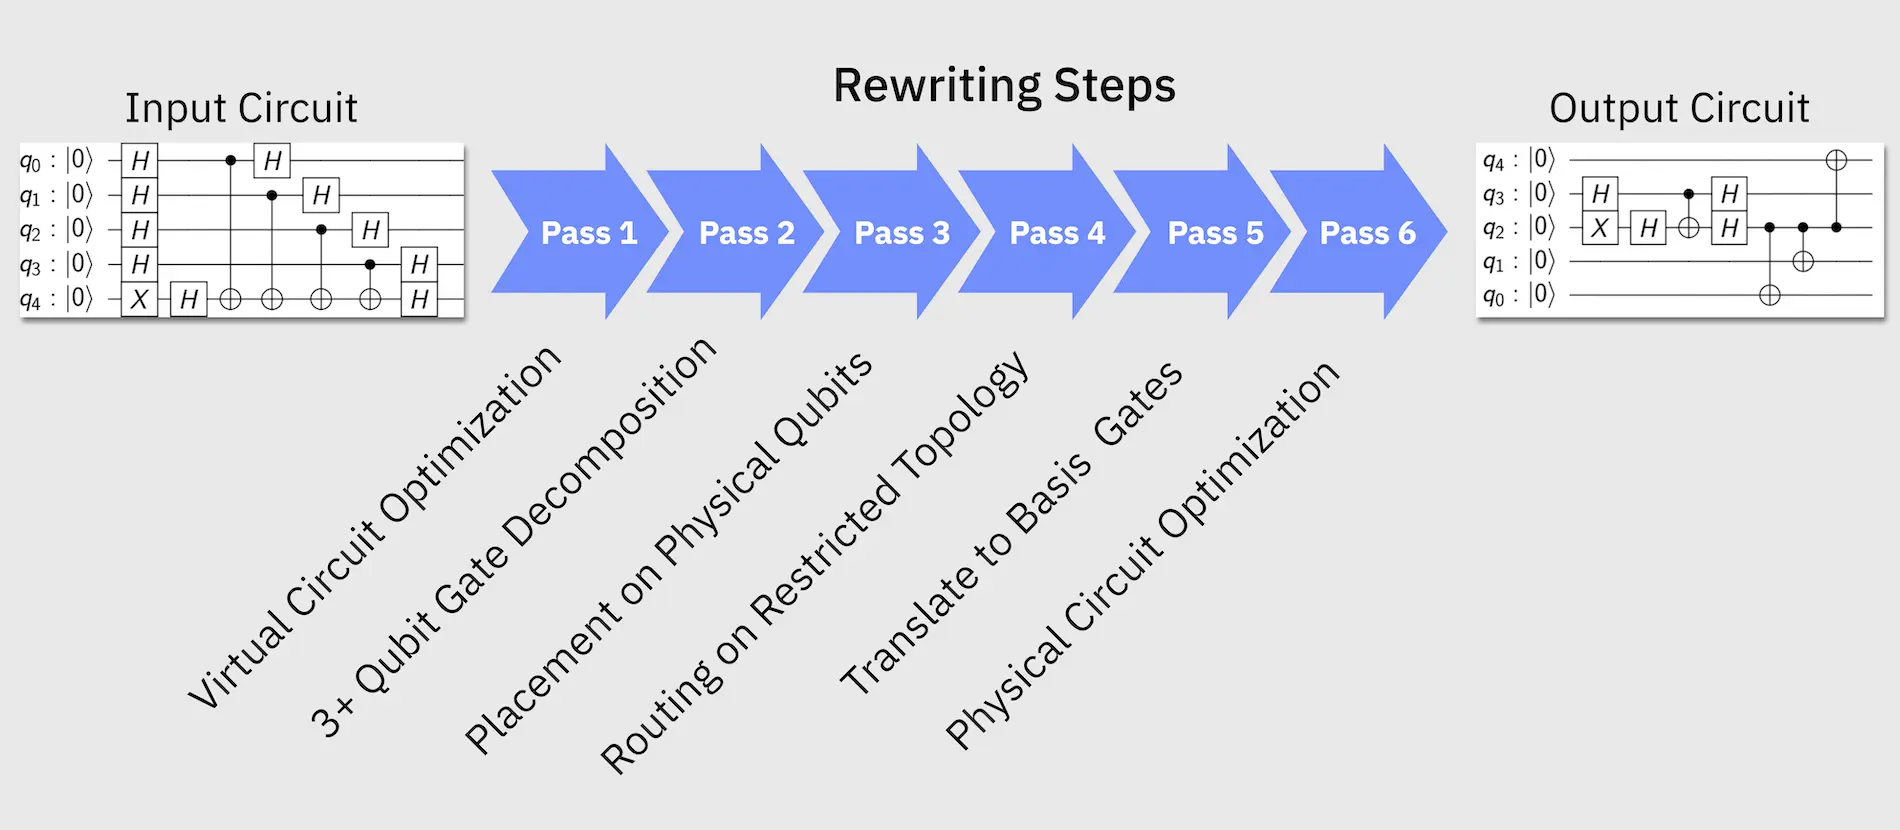
\includegraphics[width=0.75\linewidth]{image/transpiling_core_steps.png}
        \caption[Pass manager stages]{Pass manager stages. Adapted from \cite{ibmquantum_transpiler}}
        \label{fig:transpiler}
    \end{figure}
\end{enumerate}
This project will only focus on the first four stages until the translation stage.

\subsection{Initialization stage} % done chat, edited after turnitin, not yet checked
Most layout and routing algorithms only handle single- or two-qubit gates. Therefore, this stage unrolls any multi-qubit gates into sequences of single- or two-qubit gates, potentially increasing circuit size and depth \cite{ding_circuit_2020}. Two specific gates require decomposition by the backend:
\begin{enumerate}[nolistsep]
    \item A SWAP gate is decomposed into three CNOT gates, shown in Figure \ref{fig:swap-decompose}. While swap gates are essential for mapping a circuit onto the limited physical connectivity of a quantum device, they are expensive operations to execute on noisy quantum systems.
    \begin{figure}[h]
        \centering
        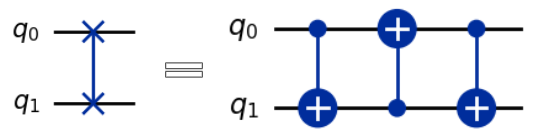
\includegraphics[width=0.5\linewidth]{image/swap decompose.png}
        \caption{Decomposed swap gate}
        \label{fig:swap-decompose}
    \end{figure}

    \item A Toffoli, also known as a controlled-controlled-not gate (CCX) gate, is a three-qubit operation. Since a Toffoli gate is not a native gate on most quantum hardware, it needs to be decomposed. The standard decomposition of a Toffoli gate involves up to 6 CNOT gates and several single-qubit gates, such as Hadamard (H) and T-gates, making it a resource-intensive process \cite{shende_toffoli_2008}, as illustrated in Figure \ref{fig:toffoli-decompose}.
    \begin{figure}[h]
        \centering
        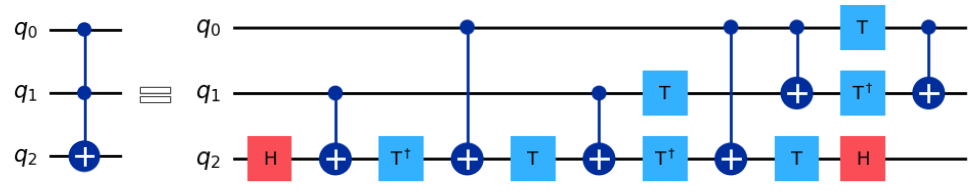
\includegraphics[width=0.6\linewidth]{image/toffoli decompose.png}
        \caption{Decomposed Toffoli gate}
        \label{fig:toffoli-decompose}
    \end{figure}
\end{enumerate}

\subsection{Layout Stage} % done chat, edited turnitin
Quantum circuits consist of quantum gates that used qubits in the computations, which must be directly mapped onto the physical qubits of a quantum device. Choosing the right initial layout is key to minimizing swap operations and reducing noise-related losses on physical qubits. This mapping, stored as a \lstinline{Layout} object, is a part of the constraints within a backend's \acrfull{isa}. For example, Figure \ref{fig:layout-placement} shows how a quantum circuit is mapped onto a device's coupling graph.
\begin{figure}[h]
    \centering
    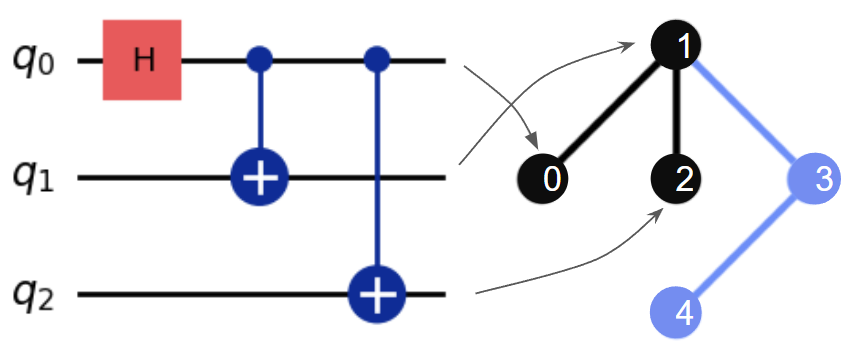
\includegraphics[width=0.5\linewidth]{image/layout_placement.png}
    \caption{Mapping logical qubits to physical qubits}
    \label{fig:layout-placement}
\end{figure}

\subsection{Routing Stage} % done chat, edited turnitin
The routing stage is a key part of the transpilation process that ensures two-qubit gates can be executed on a quantum device, considering its limited qubit connectivity. Since not all qubits on a device can interact directly, the routing stage adds SWAP gates to reposition qubits so that the required two-qubit operations are adjacent on the device's gate map \cite{wille_mqt_2023}, as shown in Figure \ref{fig:swap-placement}. Since swap gates are costly and introduce noise, minimizing their number is crucial. Qiskit uses a stochastic algorithm called \lstinline{SabreSwap} \cite{li_tackling_2019} to find an effective, though not always optimal, swap mapping. Because this method is stochastic, the resulting circuits can vary across runs, leading to different circuit depths and gate counts. \\
\begin{figure}[htb]
    \centering
    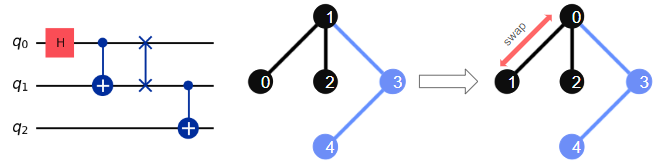
\includegraphics[width=0.7\linewidth]{image/swap_placement.png}
    \caption{Swap qubit states between physical $Q_0$ and and $Q_1$}
    \label{fig:swap-placement}
\end{figure}


\subsection{Translation Stage} % done chat, edited turnitin
When writing a quantum circuit, any arbitrary quantum gates can be used, including non-gate operations like qubit measurements and reset operations. Since most quantum devices only support a limited set of basic gates and non-gate operations, the quantum gates are translated into the native basis gates of a specific backend, which are part of the definition of a target's \acrshort{isa} \cite{gokhale_faster_2021}. For example, \lstinline{GenericBackendV2} class supports only a limited set of basic gates ['cx', 'id', 'rz', 'sx', 'x', 'reset', 'delay', 'measure'], while the quantum circuit (Figure \ref{fig:translation}) has $H$, $X$, and controlled-$P$ gates. After the transpilation process, a quantum circuit that initially had 5 logic gates is transformed into one with 12 gates.
\begin{figure}[htb]
    \centering
    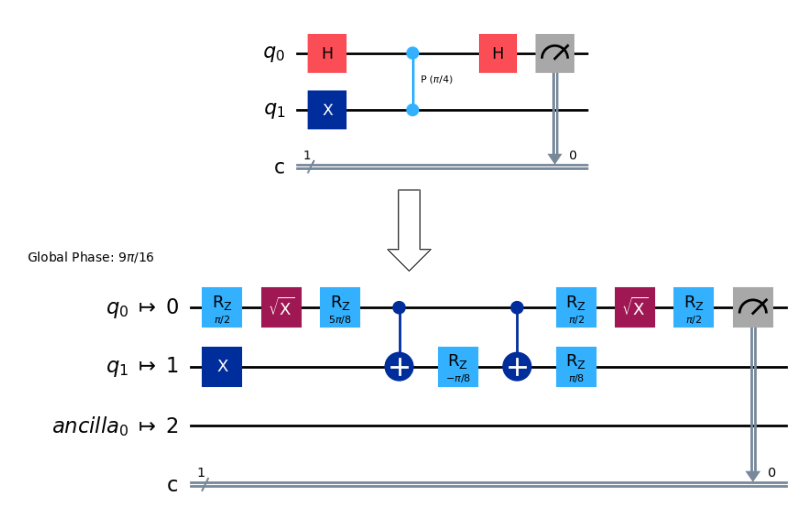
\includegraphics[width=0.7\linewidth]{image/translation_basis_gates.png}
    \caption{Translation basis gates}
    \label{fig:translation}
\end{figure}